\documentclass{article}

% Language setting
% Replace `english' with e.g. `spanish' to change the document language
\usepackage[italian]{babel}

% Set page size and margins
% Replace `letterpaper' with `a4paper' for UK/EU standard size
\usepackage[a4paper,top=2cm,bottom=2cm,left=2.5cm,right=2.5cm,marginparwidth=1.75cm]{geometry}

% Useful packages
\usepackage{amsmath}
\usepackage{graphicx}
\usepackage[colorlinks=true, allcolors=blue]{hyperref}
\usepackage{caption}
\usepackage{subcaption}
\usepackage{listings} % For code blocks
\usepackage[parfill]{parskip} % For avoiding auto indent every new line
\usepackage{tabto}
\usepackage{wrapfig} % for wrapping text and figures

\graphicspath{ {./images/} }

\title{Documentazione di progetto\\ Business Intelligence per i Servizi Finanziari}
\author{Tommaso Cammelli, 851593}

\begin{document}
\maketitle

\section{Sommario dei dati utilizzati}

\subsection{Presentazione e descrizione dei titoli selezionati}

Per questo progetto sono stati presi in considerazione 6 titoli azionari, appartenenti a 3 settori diversi:

\begin{itemize}
    \item \textbf{Settore tecnologico}: Meta Platforms, Inc. (FB), Alphabet Inc. (GOOG)
    \item \textbf{Settore militare}: Raytheon Technologies Corporation (RTX),\\ Lockheed Martin Corporation (LMT)
    \item \textbf{Settore bancario}: Bank of America Corporation (BAC), JPMorgan Chase \& Co. (JPM)
\end{itemize}

\textbf{Motivazione per scelta dei titoli}

\begin{itemize}
  \item \textbf{Meta Platforms, Inc. (FB)}: Questo titolo è stato scelto in quanto è  una delle aziende con la \emph{market capitalization} più alta nel mondo\footnote{pagina web di referenza: \href{https://companiesmarketcap.com/tech/largest-tech-companies-by-market-cap/}{https://companiesmarketcap.com/tech/largest-tech-companies-by-market-cap/}},
  e facendo parte del \emph{faang}\footnote{Acronimo dei cinque top stocks americani nel settore tecnologico, \href{https://www.investopedia.com/terms/f/faang-stocks.asp}{https://www.investopedia.com/terms/f/faang-stocks.asp}} ho ritenuto essere un investimento solido.
  considerando il recente crollo del prezzo potrebbe essere un buon momento per prendere posizioni lunghe sul titolo\footnote{\href{https://finance.yahoo.com/news/good-time-increase-meta-platforms-142109519.html}{https://finance.yahoo.com/news/good-time-increase-meta-platforms-142109519.html}}.

  \item \textbf{Alphabet Inc. (GOOG)}: Questo titolo insieme a quello precedente fa parte di \emph{faang}\footnotemark[2], è stato scelto in quanto è interessante da confrontare contro altri titoli del settore tecnologico come FB, sopratutto in momenti critici come la crisi finanziaria causata
  dall'epidemia di COVID-19, dove GOOG ha subito un crollo del 29\% nel primo trimestre\footnote{articolo riferimento declino, \href{https://www.investopedia.com/alphabet-googl-sells-off-after-revenue-decline-5072988}{https://www.investopedia.com/alphabet-googl-sells-off-after-revenue-decline-5072988}}.
  
  \item \textbf{Raytheon Technologies Corporation (RTX)}: RTX ha mostrato negli anni un trend in salita abbastanza stabile, nonostante il crollo durante la crisi finanziaria del 2020 RTX è riuscito a recuperare il crollo.\footnote{\href{https://www.investopedia.com/raytheon-technologies-drops-then-pops-on-earnings-beat-5074746}{https://www.investopedia.com/raytheon-technologies-drops-then-pops-on-earnings-beat-5074746}}.
  
  \item \textbf{Lockheed Martin Corporation (LMT)}: LMT è stata scelta in quanto è fa parte anche lui nella categoria militare e permette di confrontare l'andamento di mercato nel confronto di RTX.
  
  \item \textbf{Bank of America Corporation (BAC)}: Come primo titolo finanziario ho scelto BAC in quanto nonostante la volatilità negli ultimi anni a causa dell'epidemia, il titolo ha mostrato un leggero trend di salita negli anni ed il crollo del prezzo potrebbe
  rivelarsi una opportunità.
  
  \item \textbf{JPMorgan Chase \& Co. (JPM)}: JPM come per BAC ha risentito molto dalla crisi finanziaria del 2020, negli anni tuttavia ha mostrato un trend di salita più evidente rispetto a BAC, ritengo che potrebbe essere vantaggioso a lungo termine
\end{itemize}

\pagebreak

\subsection{Funzioni utilizzate per download e fusione}

Per il download dei dati da Yahoo! Finance\footnote{\href{https://finance.yahoo.com}{https://finance.yahoo.com}} è stata utilizzata la nota libreria di python
yfinance\footnote{Libreria FOSS per download di dati finanziari da Yahoo! finance, \href{https://pypi.org/project/yfinance/}{https://pypi.org/project/yfinance/}} dove attraverso la funzione
\verb|download()| ha permesso di scaricare i dati di interesse nel periodo rilevante per questo progetto.

\begin{lstlisting}[language=Python]
  # Esempio di download da Yahoo! Finance dello storico prezzi di FB
  import yfinance as yf

  fb_df = yf.download('FB', start='2011-11-30', end='2021-11-30')
\end{lstlisting}

Relativamente alla fusione dei dati scaricati in un unico DataFrame di Pandas\footnote{Libreria per data analysis e manipulation, 
\href{https://pandas.pydata.org/}{https://pandas.pydata.org/}} è stata utilizzata la funzione \verb|DataFrame()| 
per creare un nuovo \emph{DataFrame} vuoto, sono stati poi usati i costrutti base di python per popolare il \emph{DataFrame} con i nostri dati di interesse.

\begin{lstlisting}[language=Python]
  # Esempio di fusione dei dati da due indici scaricati precedentemente
  import pandas as pd

  adj_close_tot = pd.DataFrame()
  adj_close_tot["Meta Price"] = fb_df[["Adj Close"]]
  adj_close_tot["Alphabet Price"] = goog_df[["Adj Close"]]
\end{lstlisting}

\subsection{presentazione dei dati}

Rappresentiamo i dati ottenuti tramite un grafico a linee che si trova alla figura \ref{fig:all_stocks_price} dove 
si mostra la variazione di prezzo di tutti gli stock considerati in questo progetto\footnote{FB, GOOG, RTX, LMT, BAC, JPM} nel periodo 
da 30-11-2011 a 30-11-2021.

\begin{figure}[h]
  \centering
  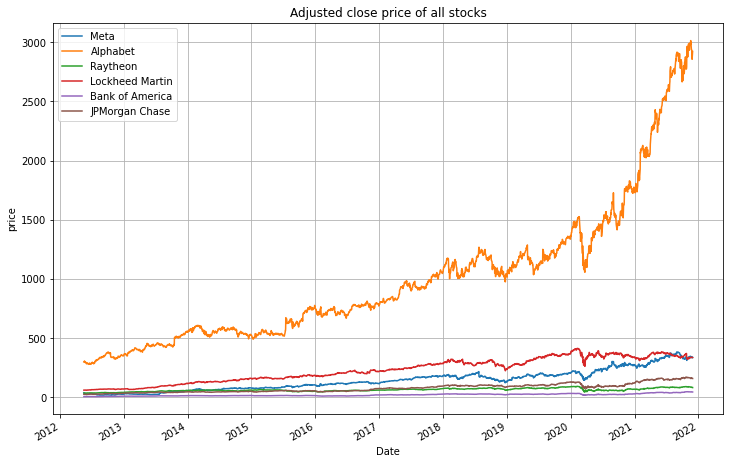
\includegraphics[width=0.7\textwidth]{all_stocks_price.png}
  \caption{grafico con prezzo degli stock da 18/05/2012 a 30/11/2021}
  \label{fig:all_stocks_price}
\end{figure}

Tutti i grafici del progetto sono stati generati utilizzando la libreria di python \emph{matplotlib}\footnote{Libreria per creare visualizzazioni dei dati anche interattive in Python, \href{https://matplotlib.org}{https://matplotlib.org}}
che tramite apposite funzioni ha permesso la quasi totale personalizzazione dei grafici per semplificare la lettura dei dati.

Rappresentiamo ora alla figura \ref{fig:all_stocks_table_10} le prime 10 righe della tabella che contiene il prezzo combinato di tutti gli stock considerati (stessa tabella utilizzata per il plot del grafico qui sopra), 
fusi in un solo \emph{DataFrame} grazie a \emph{Pandas}.

\begin{figure}[h]
  \centering
  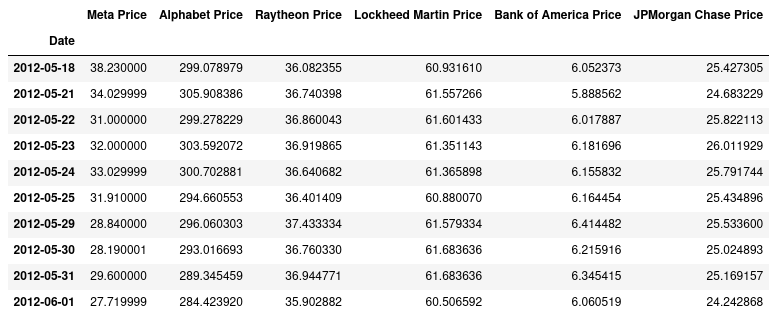
\includegraphics[width=0.7\textwidth]{stocks_combined_first_10.png}
  \caption{tabella con Adjusted Close degli stock da 18/05/2012 a 30/11/2021 (prime 10 righe)}
  \label{fig:all_stocks_table_10}
\end{figure}

\textbf{Nota:} Meta Platforms, Inc. (FB) è stata quotata in borsa solo a partire dal 18/05/2012, a causa di ciò i dati aggregati partono
solo da quella data.

%%% === Presentazione dei dati ===

\section{Statistiche descrittive}

\subsection{Rendimenti semplici e composti}

\subsubsection{Titoli Tecnologici}

Per i titoli GOOG e FB sono stati calcolati i rendimenti semplici netti (grafico a figura \ref{fig:rendimenti_semplici_tecno}) e i rendimenti compositi (grafico a figura \ref{fig:rendimenti_compositi_tecno}) e posti a confronto
si nota una generale correlazione nei rendimenti.

\begin{figure}[h]
    \centering
    \begin{minipage}{.5\textwidth}
      \centering
      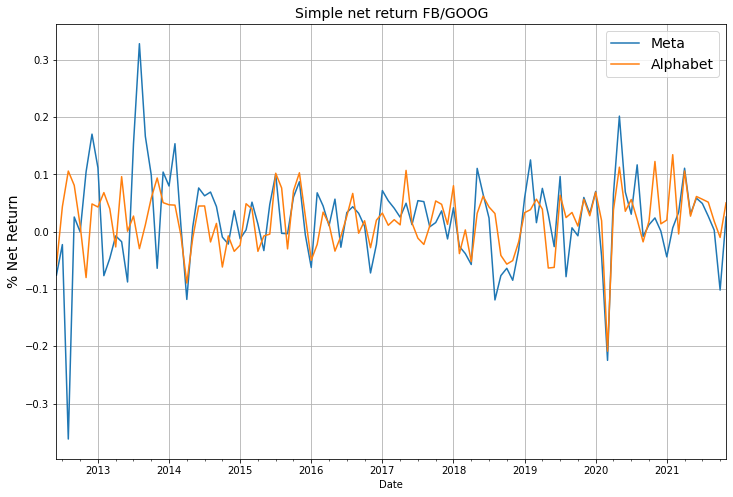
\includegraphics[width=1\linewidth]{tecno_rendimenti_semplici_netti.png}
      \captionof{figure}{Rendimenti semplici netti FB e GOOG}
      \label{fig:rendimenti_semplici_tecno}
    \end{minipage}%
    \begin{minipage}{.5\textwidth}
      \centering
      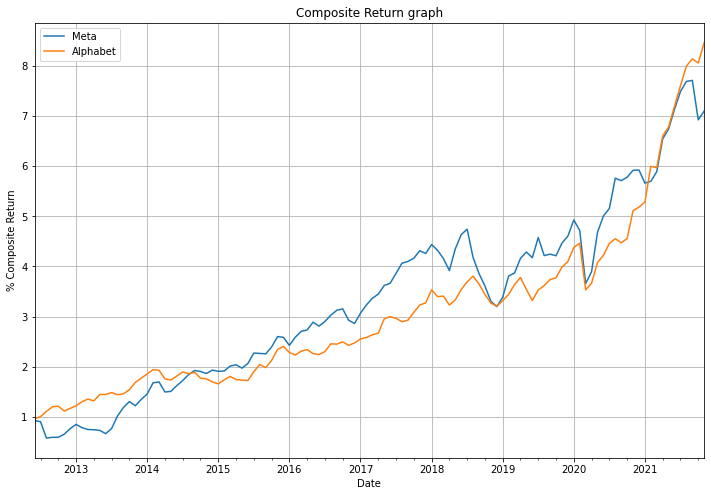
\includegraphics[width=.97\linewidth]{tecno_rendimenti_composti.png}
      \captionof{figure}{Rendimenti compositi FB e GOOG}
      \label{fig:rendimenti_compositi_tecno}
    \end{minipage}
\end{figure}

\textbf{Note sui titoli tecnologici}

Confrontando le serie storiche di GOOG e FB nel grafico a figura \ref{fig:all_stocks_price}, utilizzando la funzione \verb|.corr()| di pandas si mostra un forte correlazione positiva di \verb|0.962272| (figura \ref{fig:corr_tecno})
tra i due titoli, come dimostrato anche dai simili rendimenti compositi (ad eccezione per alcuni eventi).

\begin{figure}[h]
  \centering
  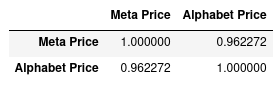
\includegraphics[width=0.4\textwidth]{corr_tecno.png}
  \caption{tabella con correlazione titoli GOOG e FB (metodo di Pearson)}
  \label{fig:corr_tecno}
\end{figure}

\pagebreak

\textbf{Note sui rendimenti di Meta (FB)}

Osservando il grafico in figura \ref{fig:rendimenti_semplici_tecno} relativamente ai rendimenti semplici di FB, notiamo \textbf{3} eventi di notevole discostamento dalla media.

Nel primo trimestre del 2012 si nota un significativo crollo, analizzando notizie e articoli si può ricondurre il crollo a scetticismo che c`è stato
tra gli investitori\footnote{\href{https://money.cnn.com/2012/05/22/markets/facebook-shares/index.htm}{https://money.cnn.com/2012/05/22/markets/facebook-shares/index.htm}} in quanto
Facebook (ora Meta) all'epoca era stata appena quotata in borsa, il crollo è stato circa del 35\% solo nei primi mesi.

Nel terzo trimestre del 2013 tuttavia viene evidenziato una crescita sostanziale rispetto alla media, nonostante il crollo capitato poco dopo la quotazione in borsa nel 2012,
a metà anno il prezzo di FB è riuscito a raggiungere di nuovo il prezzo di \emph{IPO}\footnote{Initial Public Offering, \href{https://www.investopedia.com/terms/i/ipo.asp}{https://www.investopedia.com/terms/i/ipo.asp}}
raggiungendo poi verso il terzo trimestre la quota record del tempo di 50\$, in base a vari 
articoli\footnote{
  \href{https://www.reuters.com/article/us-facebook-ipoprice-idUSBRE96T1CI20130730}{https://www.reuters.com/article/us-facebook-ipoprice-idUSBRE96T1CI20130730},
  
  \hspace{1.5mm} \href{https://money.cnn.com/2013/09/26/investing/facebook-stock/index.html}{https://money.cnn.com/2013/09/26/investing/facebook-stock/index.html}
  }
si evidenzia come la crescita possa essere attribuita dalla introduzione delle pubblicità su dispositivi mobile (precedentemente la pubblicità era mostrata solo da sito web),
a luglio 2013 facebook ha infatti annunciato che la pubblicità su mobile ha contribuito al 41\% delle loro vendite nel secondo semestre.

Tra il primo ed il secondo trimestre del 2020, come evidenziato dal grafico c'è stato un grande discostamento dalla media, inizialmente molto negativo ma poco dopo molto positivo,
la caduta inziale del prezzo la si può attribuire alla crisi finanziaria del 2020, scatenata dalla epidemia da 
covid-19\footnote{
  \href{https://www.investopedia.com/facebook-stock-crashes-into-bear-market-territory-4800598}{https://www.investopedia.com/facebook-stock-crashes-into-bear-market-territory-4800598}
}.\\
Tuttavia grazie alla natura digitale del servizio, dunque non esposta alla epidemia come altre attività e all'annuncio di \emph{Facebook Shops} il prezzo ha velocemente raggiunto il valore pre-crollo arrivando
addirittura ad un record del tempo (20-05-2020) di 
\$230.75\footnote{
  \href{https://www.cnbc.com/2020/05/20/facebook-shares-reach-all-time-high-after-announcing-online-shopping-feature.html}{https://www.cnbc.com/2020/05/20/facebook-shares-reach-all-time-high-after-announcing-online-shopping-feature.html}
}\\

\textbf{Note sui rendimenti di Alphabet (GOOG)}

Sul titolo GOOG si notano distaccamenti negativi sul rendimento di entità notevolmente inferiore rispetto a FB, tuttavia si hanno distaccamenti positivi più numerosi (il net return raggiunge 0.1 più volte rispetto a FB) anche se spesso non oltre 0.1.

Come per FB, ad aprile 2020 c'è stato un decremento significativo del prezzo (che si è riflettuto sul rendimento) a causa della epidemia da 
covid-19\footnote{
  \href{https://www.investopedia.com/alphabet-stock-crashes-into-bear-market-territory-4800600}{https://www.investopedia.com/alphabet-stock-crashes-into-bear-market-territory-4800600}
}
, ma sempre per il fatto che Alphabet Inc. fornisce
prevalentemente servizi digitali il prezzo è ritornato al valore pre-crollo velocemente.

\subsubsection{Titoli Militari}

Per i titoli RTX e LMT sono stati calcolati i rendimenti semplici netti (grafico a figura \ref{fig:rendimenti_semplici_mil}) e i rendimenti compositi (grafico a figura \ref{fig:rendimenti_compositi_mil}) e posti a confronto
si nota una generale correlazione nei rendimenti, anche se di entità inferiore rispetto a FB/GOOG.

\begin{figure}[h]
  \centering
  \begin{minipage}{.5\textwidth}
    \centering
    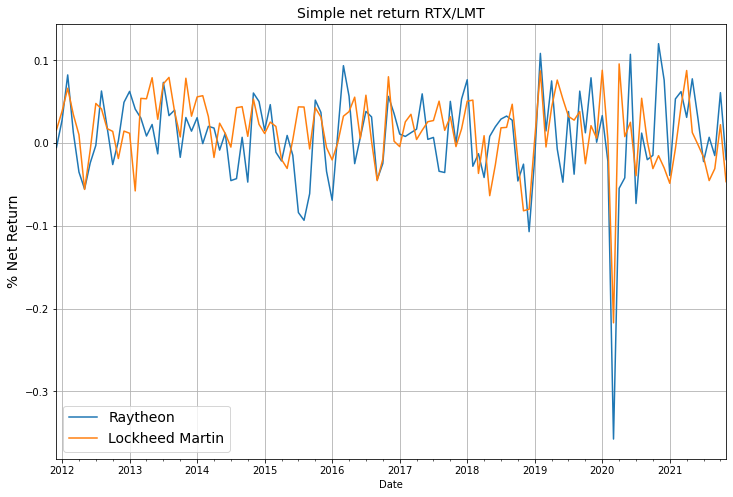
\includegraphics[width=1\linewidth]{mil_rendimenti_semplici_netti.png}
    \captionof{figure}{Rendimenti semplici netti RTX e LMT}
    \label{fig:rendimenti_semplici_mil}
  \end{minipage}%
  \begin{minipage}{.5\textwidth}
    \centering
    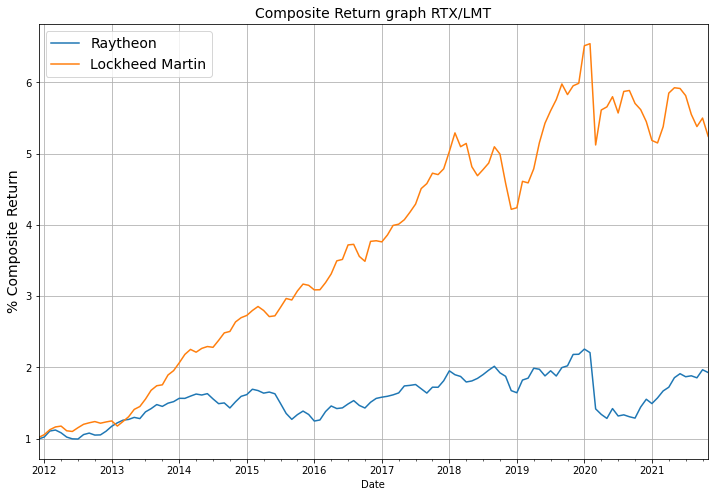
\includegraphics[width=.97\linewidth]{mil_rendimenti_composti.png}
    \captionof{figure}{Rendimenti compositi RTX e LMT}
    \label{fig:rendimenti_compositi_mil}
  \end{minipage}
\end{figure}

Confrontando i titoli RTX e LMT usando sempre il grafico a figura \ref{fig:all_stocks_price} e utilizzando la funzione \verb|.corr()| di pandas
viene mostrata anche in questo caso una \textbf{forte correlazione positiva} di \verb|0.836831| (figura \ref{fig:corr_mill}).

\begin{figure}[h]
  \centering
  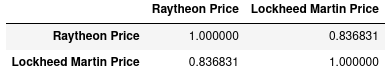
\includegraphics[width=0.4\textwidth]{corr_mil.png}
  \caption{tabella con correlazione titoli RTX e LMT (metodo di Pearson)}
  \label{fig:corr_mill}
\end{figure}

\textbf{Note sui rendimenti di Raytheon (RTX)}

Osservando il grafico in figura \ref{fig:rendimenti_semplici_mil} relativamente ai rendimenti semplici di RTX, si nota come il nel tempo è
stato molto fluido, troviamo \textbf{3} eventi notevoli.

Sul titolo RTX è stato più complicato la ricerca di notizie coerenti con il crollo del prezzo in quanto è notevolmente meno famoso rispetto a FB o GOOG,
tuttavia relativamente al primo ed al secondo crollo si può assumere siano in relazione alla politica di export delle armi americane.

Il crollo più notevole è accaduto durante la crisi finanziaria del 2020, in base a un 
articolo\footnote{
  \href{https://www.fool.com/investing/2020/07/02/heres-why-raytheon-technologies-shares-are-down-34.aspx}{https://www.fool.com/investing/2020/07/02/heres-why-raytheon-technologies-shares-are-down-34.aspx}
}
la motivazione del crollo è stata a causa della temporanea debolezza nel settore commerciale aerospaziale, causata dalla epidemia da COVID-19,
si assume comunque che essendo una compagnia incentrata nel settore aerospaziale sarà comunque una migliore scelta rispetto alla competizione per il
settore della difesa.\\

\textbf{Note sui rendimenti di Lockheed Martin (LMT)}

Il titolo LMT ha subito variazioni molto meno significanti rispetto a RTX e gli altri titoli (come si può vedere dal grafico a figura \ref{fig:rendimenti_semplici_mil}), analizzando varie notizie nel web si identificano \textbf{2} eventi significativi.

Tra fine 2018 e l'inizio del 2019 si è registrato un crollo del 18.4\% relativo allo stock LMT, in base ad un 
articolo\footnote{
  \href{https://www.fool.com/investing/2019/01/11/heres-why-lockheed-martin-lost-184-in-2018.aspx}{https://www.fool.com/investing/2019/01/11/heres-why-lockheed-martin-lost-184-in-2018.aspx}
}
le cause del crollo sono molteplici, uno delle cause identificate è una continua diminuzione del budget dalla casa bianca, una altra è la dimissione improvvisa del 
CFO\footnote{
  Chief Financial Officer, \href{https://en.wikipedia.org/wiki/Chief_financial_officer}{https://en.wikipedia.org/wiki/Chief\_financial\_officer}
}
in quanto era ben visto dagli investitori per le sue abilità comunicative.

Il crollo più importante del prezzo è stato durante la crisi finanziaria del 2020, dopo il crollo nel primo trimestre tuttavia c'è stato un notevole recupero poco dopo messo poi a rischio verso ottobre a causa di problemi nella supply chain della
produzione\footnote{
  \href{https://www.investopedia.com/lockheed-martin-lmt-sells-off-despite-strong-quarter-5083204}{https://www.investopedia.com/lockheed-martin-lmt-sells-off-despite-strong-quarter-5083204}
}
causato dal tilt nelle fabbriche e nei trasporti.

Nello stesso articolo si evidenzia inoltre come la motivazione della instabilità verso la fine del 2020 sia anche causata da una incertezza politica, in quanto si assumeva che una vittoria democratica avrebbe tagliato il
budget alla difesa, anche se il rischio di guerra nucleare dovrebbe evitare un crollo del titolo.

\subsubsection{Titoli Bancari}

Per i titoli BAC e JPM sono stati calcolati i rendimenti semplici netti (grafico a figura \ref{fig:rendimenti_semplici_banc}) e i rendimenti composti (grafico a figura \ref{fig:rendimenti_compositi_banc}) e posti a confronto
anche per questi due titoli si nota una forte correlazione nei rendimenti.

\begin{figure}[h]
  \centering
  \begin{minipage}{.5\textwidth}
    \centering
    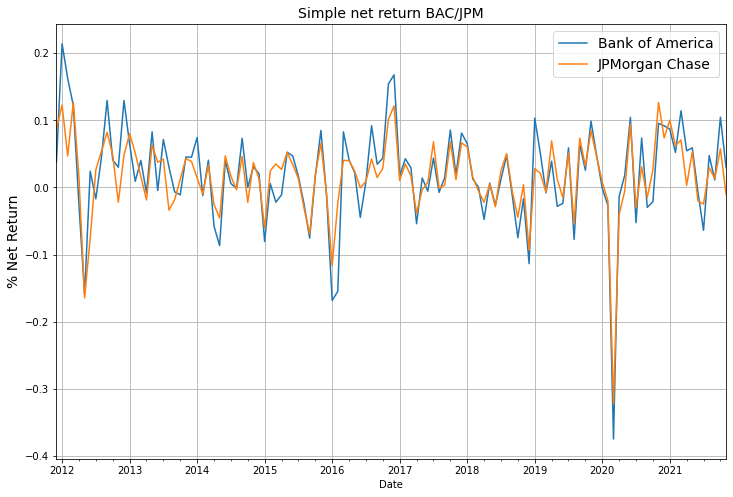
\includegraphics[width=1\linewidth]{banc_rendimenti_semplici_netti.png}
    \captionof{figure}{Rendimenti semplici netti BAC e JPM}
    \label{fig:rendimenti_semplici_banc}
  \end{minipage}%
  \begin{minipage}{.5\textwidth}
    \centering
    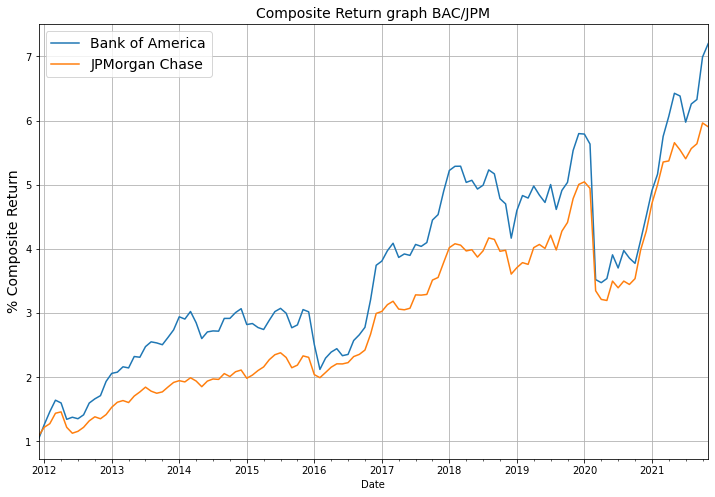
\includegraphics[width=.97\linewidth]{banc_rendimenti_composti.png}
    \captionof{figure}{Rendimenti compositi BAC e JPM}
    \label{fig:rendimenti_compositi_banc}
  \end{minipage}
\end{figure}

Confrontando i titoli BAC e JPM usando il grafico a figura \ref{fig:all_stocks_price} e utilizzando la funzione \verb|.corr()| di pandas
viene mostrata una \textbf{forte correlazione positiva} di \verb|0.909522| (figura \ref{fig:corr_banc}).

\begin{figure}[h]
  \centering
  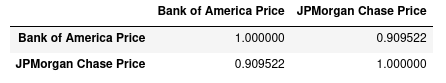
\includegraphics[width=0.4\textwidth]{corr_banc.png}
  \caption{tabella con correlazione titoli BAC e JPM (metodo di Pearson)}
  \label{fig:corr_banc}
\end{figure}

\textbf{Note sui rendimenti di Bank of America (BAC)}

Il titolo BAC ha in multiple occasioni dei sostanziali aumenti di prezzo ma anche dei crolli, identifichiamo almeno \textbf{5} eventi notevoli.

Nel primo trimestre del 2012 si nota un netto crollo del prezzo, facendo delle ricerche ho trovato un 
articolo\footnote{
  \href{https://www.reuters.com/article/uk-bofa-lawsuit-idUKBRE88R11X20120928}{https://www.reuters.com/article/uk-bofa-lawsuit-idUKBRE88R11X20120928}
}
che spiega come BAC ha accettato di pagare 2.3 milioni di dollari agli investitori per patteggiare una causa legale per gli eventi legati alla crisi finanziaria del 2008.
Essendo un periodo vicino al 2008 si assume anche che la alta volatilità si anche data dalla poca fiducia degli investitori in questo titolo.

Nel 2016 si registra un altro periodo di instabilità per questo titolo, risultato poi verso la fine dell'anno con un aumento del 34\% sul prezzo,
secondo questo 
articolo\footnote{
  \href{https://www.fool.com/investing/2016/12/29/why-bank-of-americas-stock-climbed-34-in-2016.aspx}{https://www.fool.com/investing/2016/12/29/why-bank-of-americas-stock-climbed-34-in-2016.aspx}
}
il declino del prezzo all'inizio dell'anno è stato a causa del crollo dei prezzi relativi all'energia,
successivamente i prezzi del settore energetico ci hanno messo poco tempo a recuperare, tuttavia nonostante il recupero a metà anno il prezzo di BAC è comunque sceso,
la causa della seconda declinazione dei prezzi, si può attribuire alla improvvisa decisione dell'inghilterra di uscire dalla unione europea (brexit), che ha causato un momento
di incertezza finanziaria, sopratutto con Bank of America in quanto a causa di brexit avrebbe dovuto spostare parte delle proprie operazioni in un altro paese europeo.\\
Verso la fine dell'anno poi c'è stato una crescita notevole e inaspettata del prezzo, secondo l'articolo questa crescita può essere stata a causa della vittoria del partito
Repubblicano delle elezioni presidenziali, in quanto il candidato presidente aveva promesso la rimozione di regolatorie instaurate nel 2010 dal precedente Presidente.

Nel 2020 come per i titoli mostrati in precedenza c'è stato un grosso crollo del prezzo di BAC a causa della crisi finanziaria del 2020, secondo questo 
articolo\footnote{
  \href{https://www.investopedia.com/bank-of-america-earnings-4770948}{https://www.investopedia.com/bank-of-america-earnings-4770948}
}
nonostante l'ottimismo del CEO riguardante il futuro recupero dal crollo, i mesi successivi sono rimasti altamente instabili e non hanno portato come per i titoli tecnologici
a un aumento stabile.\\

\textbf{Note sui rendimenti di JPMorgan Chase (JPM)}

Controllando i grafici relativi al prezzo e rendimenti, si può notare come il titolo JPM sia stato molto correlato con BAC, in quanto operano nello stesso settore e sono entrambi
titoli finanziari.\\
Relativamente agli eventi del 2012 e 2016 si può assumere che gli stessi eventi di BAC abbiano causato il crollo sui rendimenti e quindi periodi di instabilità.

Relativamente alla crisi finanziaria del 2020, secondo questo
articolo\footnote{
  \href{https://www.cnbc.com/2020/04/14/jpmorgan-chase-jpm-earnings-q1-2020.html}{https://www.cnbc.com/2020/04/14/jpmorgan-chase-jpm-earnings-q1-2020.html}
}
oltre al crollo del prezzo a causa della epidemia, c'è stato un enorme movimento di 6.8 milioni di dollari alla riserva di credito della banca, movimento che si assume sia stato effettuato
per proteggere la banca da un aumento di default relativi alle attività che hanno effettuato prestiti con JPM, questo movimento ha causato un ulteriore crollo del prezzo che si è propagato nei mesi successivi.

\pagebreak

\subsection{Istogrammi sui rendimenti e dispersione}

Per misurare la dispersione sui titoli ci torna utile il concetto di deviazione standard, grazie ad essa si può avere una idea della
 volatilità associata al titolo, un dato utile per effettuare investimenti e/o strategie di 
trading\footnote{
  \href{https://www.investopedia.com/terms/s/standarddeviation.asp}{https://www.investopedia.com/terms/s/standarddeviation.asp}
}.\\

\subsubsection{Titoli tecnologici (Meta/Alphabet)}

L'istogramma del rendimento relativo ai titoli GOOG e FB può essere visto a figura \ref{fig:isto_rendimenti_tecno}, mentre la distribuzione dei 
rendimenti si trova nel grafico in figura \ref{fig:dispersione_tecno}.
Dai dati si evidenzia come la maggior parte dei rendimenti avviene tra \verb|0.0| e \verb|0.1|, oltre al fatto che alphabet nel periodo di interesse ha avuto rendimenti più alti
rispetto a Meta.

\begin{figure}[h]
  \centering
  \begin{minipage}{.5\textwidth}
    \centering
    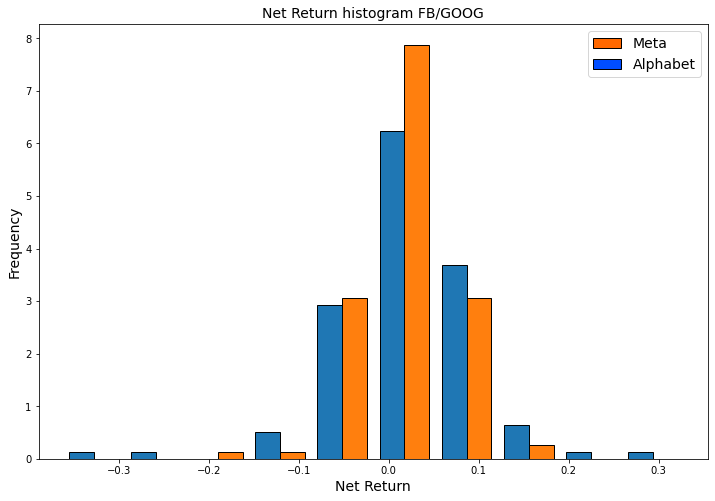
\includegraphics[width=1\linewidth]{net_ret_tecno_hist.png}
    \captionof{figure}{Istogramma rendimenti FB e GOOG}
    \label{fig:isto_rendimenti_tecno}
  \end{minipage}%
  \begin{minipage}{.5\textwidth}
    \centering
    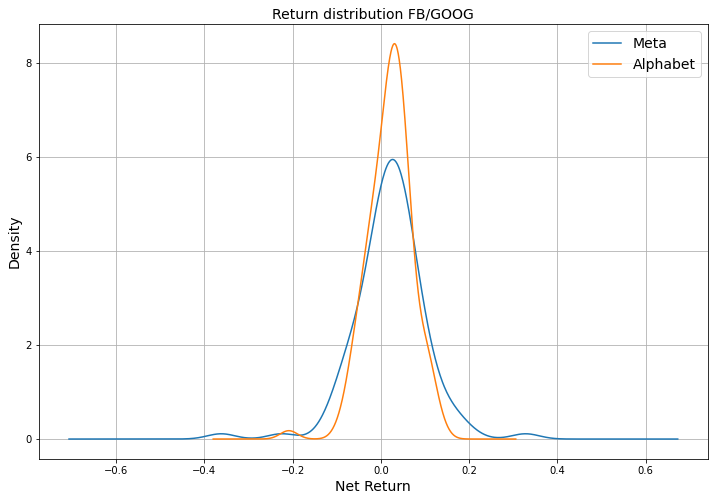
\includegraphics[width=1\linewidth]{dispersione_tecno.png}
    \captionof{figure}{Dispersione di FB e GOOG}
    \label{fig:dispersione_tecno}
  \end{minipage}
\end{figure}

Inoltre é stata calcolata grazie a \emph{Pandas} la Deviazione Standard, dove il risultato si può vedere nella tabella a figura \ref{fig:ds_tecno}.

\begin{figure}[h]
  \centering
  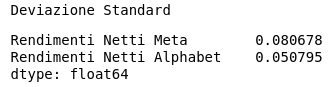
\includegraphics[width=0.4\textwidth]{ds_tecno.png}
  \caption{Deviazione Standard dei titoli FB e GOOG}
  \label{fig:ds_tecno}
\end{figure}

\subsubsection{Titoli militari (Raytheon/Lockheed Martin)}

L'istogramma del rendimento relativo ai titoli RTX e LMT può essere visto nel grafico a figura \ref{fig:isto_rendimenti_mil}, mentre la distribuzione dei rendimenti
si trova nel grafico a figura \ref{fig:dispersione_mil}.\\
Dai dati si evidenzia che i rendimenti si trovano per la maggior parte tra \verb|-0.05| e \verb|0.5|, Lockheed martin ha avuto rendimenti più alti rispetto
a Raytheon.

\begin{figure}[h]
  \centering
  \begin{minipage}{.5\textwidth}
    \centering
    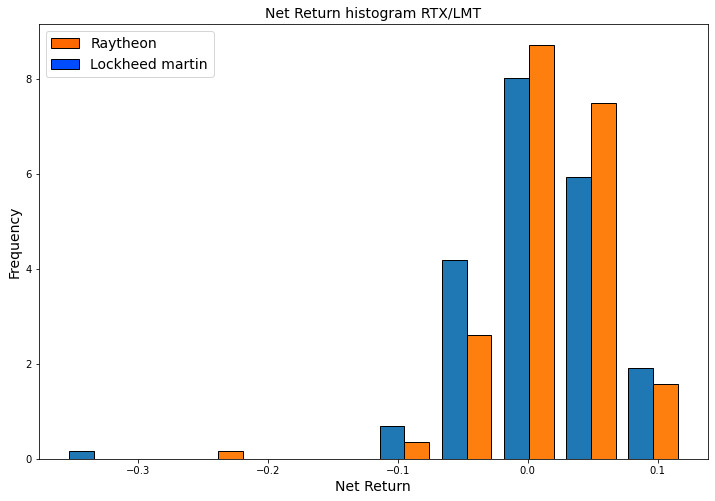
\includegraphics[width=1\linewidth]{net_ret_mil_hist.png}
    \captionof{figure}{Istogramma rendimenti RTX e LMT}
    \label{fig:isto_rendimenti_mil}
  \end{minipage}%
  \begin{minipage}{.5\textwidth}
    \centering
    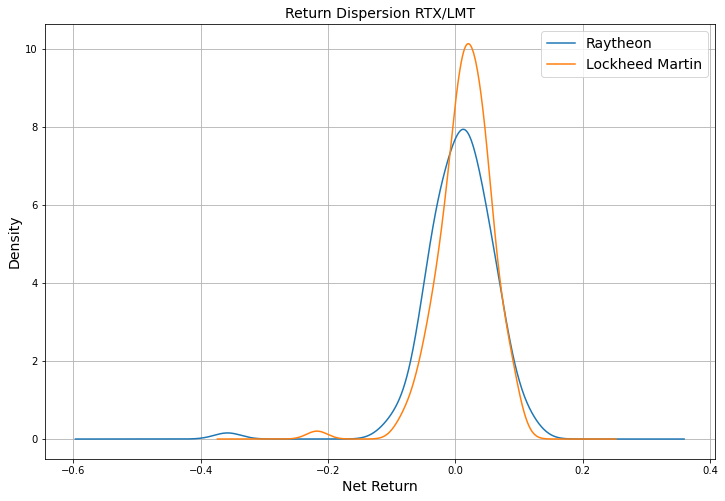
\includegraphics[width=1\linewidth]{dispersione_mil.png}
    \captionof{figure}{Dispersione di RTX e LMT}
    \label{fig:dispersione_mil}
  \end{minipage}
\end{figure}

Sempre con \emph{pandas} è stata calcolata la Deviazione Standard, dove il risultato è riportato nella tabella a figura \ref{fig:ds_mil}.

\begin{figure}[h]
  \centering
  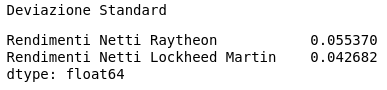
\includegraphics[width=0.4\textwidth]{ds_mil.png}
  \caption{Deviazione Standard dei titoli RTX e LMT}
  \label{fig:ds_mil}
\end{figure}

\pagebreak

\subsubsection{Titoli bancari (Bank of America/JPMorgan Chase)}

L'istogramma per il rendimento dei titoli finanziari BAC e JPM si può vedere nel grafico nella figura \ref{fig:isto_rendimenti_banc}, mentre la distribuzione dei rendimenti
si può vedere nel grafico in figura \ref{fig:dispersione_banc}.\\
Dai dati si evidenzia che i rendimenti si trovano per la maggior parte tra \verb|-0.01| e \verb|0.1|, Bank of America ha avuto rendimenti più alti
rispetto a JPMorgan Chase.

\begin{figure}[h]
  \centering
  \begin{minipage}{.5\textwidth}
    \centering
    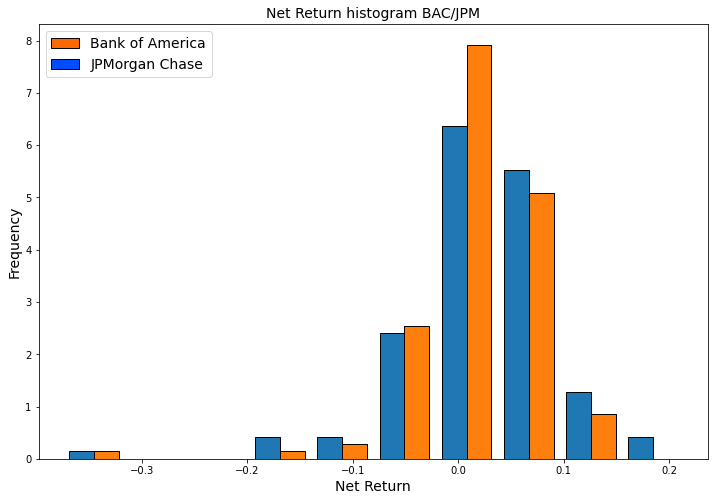
\includegraphics[width=1\linewidth]{net_ret_banc_hist.png}
    \captionof{figure}{Istogramma rendimenti BAC e JPM}
    \label{fig:isto_rendimenti_banc}
  \end{minipage}%
  \begin{minipage}{.5\textwidth}
    \centering
    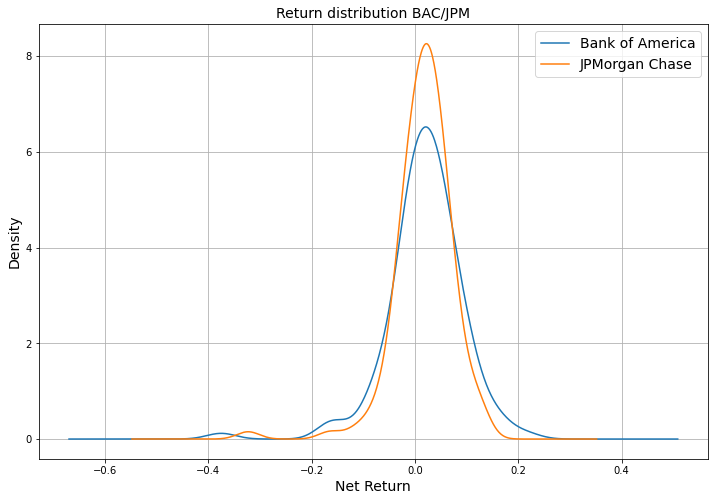
\includegraphics[width=1\linewidth]{dispersione_banc.png}
    \captionof{figure}{Dispersione di BAC e JPM}
    \label{fig:dispersione_banc}
  \end{minipage}
\end{figure}

Con \emph{pandas} è stata calcolata la Deviazione Standard, dove il risultato è nella tabella a figura \ref{fig:ds_banc}.

\begin{figure}[h]
  \centering
  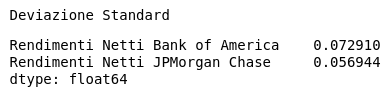
\includegraphics[width=0.4\textwidth]{ds_banc.png}
  \caption{Deviazione Standard dei titoli BAC e JPM}
  \label{fig:ds_banc}
\end{figure}

\pagebreak

\subsection{Grafici diagnositici a 4 sezioni}

Vengono mostrati per i titoli considerati la serie di 4 grafici diagnostici (Istogramma, kernel density, qq-plot e boxplot).\\
Questi grafici rappresentano 4 modi diversi per rappresentare la \textbf{Distribuzione Normale}, fondamentale per studiare la distribuzione sui rendimenti dei titoli.

\subsubsection{Grafici Diagnostici per Meta Platforms, Inc. (FB)}

Per Meta, possiamo trovare i grafici alla figura \ref{fig:meta_diagn}, si può notare come i rendimenti sono distribuiti normalmente e simmetricamente,
Si notano inoltre degli outliners: due tra \verb|0.2| e \verb|0.35| e due tra \verb|-0.2| e \verb|-0.4|.

\begin{figure}[h]
  \centering
  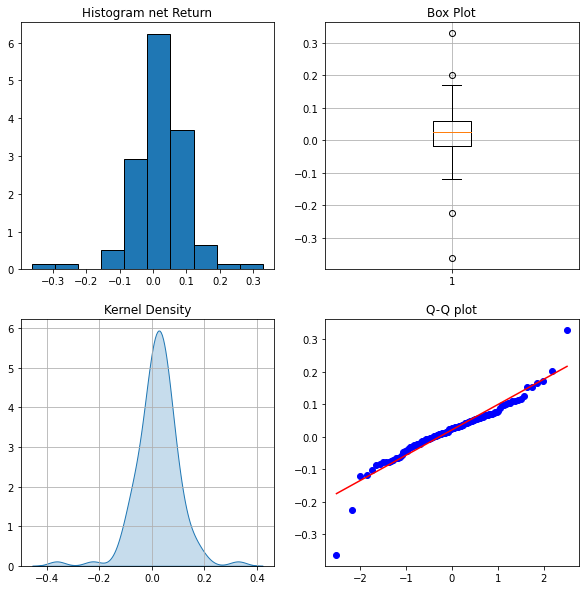
\includegraphics[width=0.7\textwidth]{meta_diagn.png}
  \caption{Grafici diagnostici per Meta (FB)}
  \label{fig:meta_diagn}
\end{figure}

\pagebreak

\subsubsection{Grafici Diagnostici per Alphabet Inc. (GOOG)}

Per Alphabet, possiamo trovare i grafici alla figura \ref{fig:goog_diagn}, possiamo notare anche qui che i rendimenti sono distribuiti normalmente, con una notevole inclinazione positiva rispetto a FB,
Anche per questo titolo si nota un outliner: tra \verb|-0.20| e \verb|-0.25|.

\vspace{3cm}

\begin{figure}[h]
  \centering
  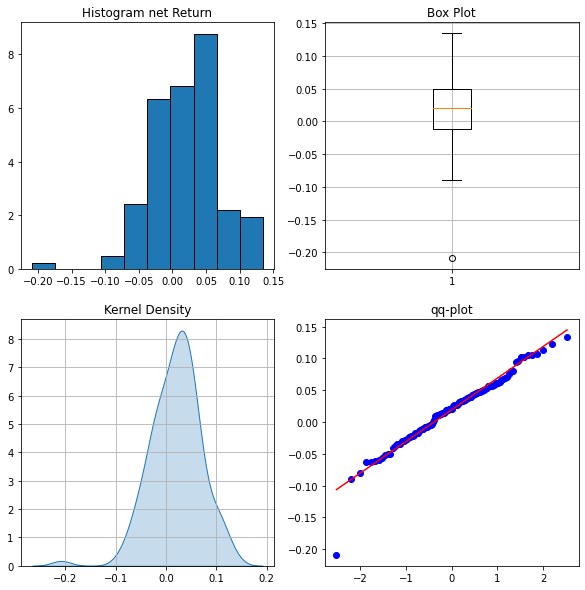
\includegraphics[width=0.7\textwidth]{goog_tecn.png}
  \caption{Grafici diagnostici per Alphabet (GOOG)}
  \label{fig:goog_diagn}
\end{figure}

\pagebreak

\subsubsection{Grafici Diagnostici per Raytheon Technologies Corporation. (RTX)}

Per Raytheon, i grafici si trovano alla figura \ref{fig:rtx_diagn}, possiamo notare che qui i rendimenti sono distribuiti normalmente e simmetricamente.
Per questo titolo troviamo un outliner: tra \verb|-0.35| e \verb|-0.4|.

\vspace{3cm}

\begin{figure}[h]
  \centering
  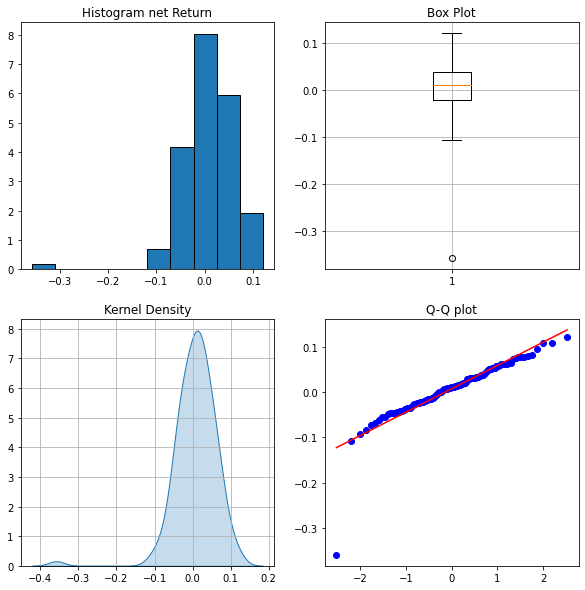
\includegraphics[width=0.7\textwidth]{rtx_diagn.png}
  \caption{Grafici diagnostici per Raytheon (RTX)}
  \label{fig:rtx_diagn}
\end{figure}

\pagebreak

\subsubsection{Grafici Diagnostici per Lockheed Martin Corporation. (LMT)}

Per Lockheed Martin, i grafici si trovano alla figura \ref{fig:lmt_diagn}, anche qui i rendimenti sono distribuiti normalmente e in maniera simmetrica (la curva è più translata verso destra).
Per questo titoli abbiamo tre outliner: due tra \verb|-0.05| e \verb|-0.10|, e uno tra \verb|-0.20| e \verb|-0.25|.

\vspace{3cm}

\begin{figure}[h]
  \centering
  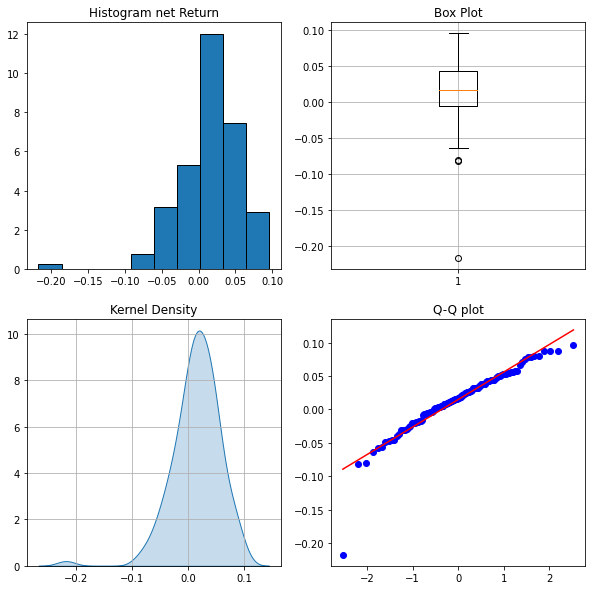
\includegraphics[width=0.7\textwidth]{lmt_diagn.png}
  \caption{Grafici diagnostici per Lockheed Martin (LMT)}
  \label{fig:lmt_diagn}
\end{figure}

\pagebreak

\subsubsection{Grafici Diagnostici per Bank of America. (BAC)}

Per Bank of America, i grafici diagnostici sono alla figura \ref{fig:bac_diagn}, anche qui sono distribuiti generalmente normalmente e simmetricamente.
Per BAC abbiamo numerosi outliners: tre tra \verb|0.15| e \verb|0.25|, quattro o più tra \verb|-0.1| e \verb|-0.2| e uno tra \verb|-0.35| e \verb|-0.4|.

\vspace{3cm}

\begin{figure}[h]
  \centering
  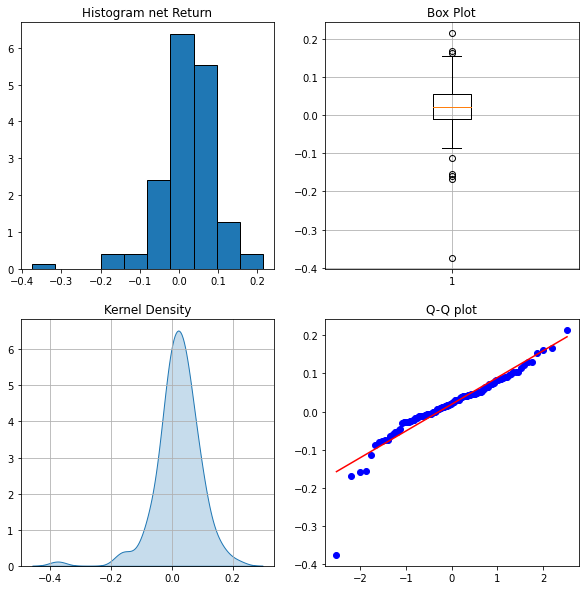
\includegraphics[width=0.7\textwidth]{bac_diagn.png}
  \caption{Grafici diagnostici per Bank of America (BAC)}
  \label{fig:bac_diagn}
\end{figure}

\pagebreak

\subsubsection{Grafici Diagnostici per JPMorgan Chase. (JPM)}

Per JPMorgan Chase, troviamo i grafici diagnostici alla figura \ref{fig:jpm_diagn}, la distribuzione è anche qui normale e leggermente inclinata verso destra.
Per questo titolo abbiamo 3 outliners: due tra \verb|-0.1| e \verb|-0.2| e uno tra \verb|-0.3| e \verb|-0.35|.

\vspace{3cm}

\begin{figure}[h]
  \centering
  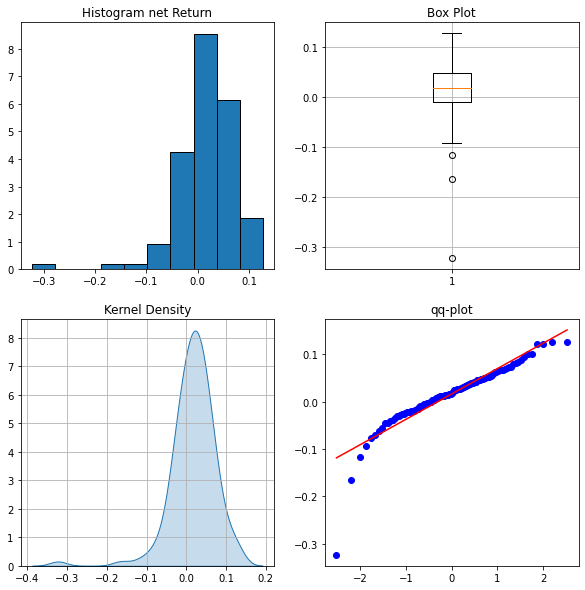
\includegraphics[width=0.7\textwidth]{jpm_diagn.png}
  \caption{Grafici diagnostici per JPMorgan Chase (JPM)}
  \label{fig:jpm_diagn}
\end{figure}

\pagebreak

\subsection{Statistiche descrittive univariate}

Per ogni serie di rendimenti sono state considerate le seguenti statistiche univariate: media, varianza, deviazione standard, asimmetria e curtosi.

Tali statistiche univariate servono per [TODO]

\textbf{Statistiche per Meta (FB)}

Per Meta identifichiamo una volatilità del \verb|36.44|\%, i grafici e la tabella sono a figura \ref{fig:fb_stats} e \ref{fig:fb_vol}.

\begin{figure}[h]
  \centering
  \begin{minipage}{.5\textwidth}
    \centering
    \vspace{4.35cm}
    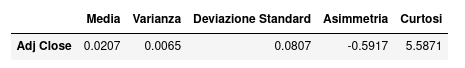
\includegraphics[width=1\linewidth]{meta_stats.png}
    \captionof{figure}{Statistiche univariate per Meta (FB)}
    \label{fig:fb_stats}
  \end{minipage}%
  \begin{minipage}{.5\textwidth}
    \centering
    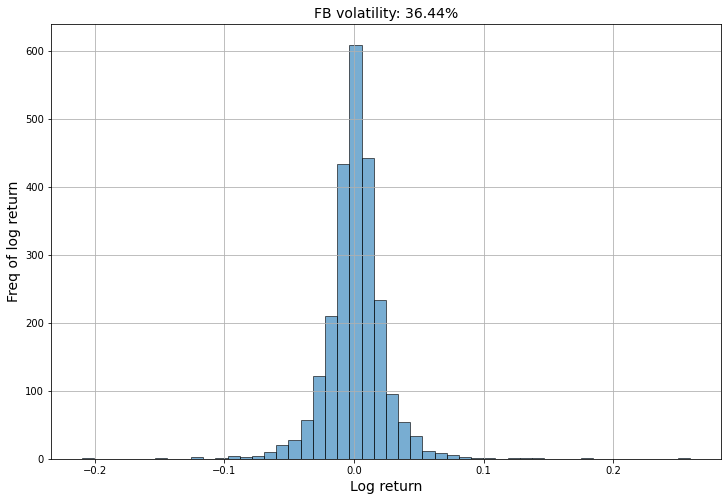
\includegraphics[width=1\linewidth]{meta_volatility.png}
    \captionof{figure}{Grafico volatilità di Meta (FB)}
    \label{fig:fb_vol}
  \end{minipage}
\end{figure}

\textbf{Statistiche per Alphabet (GOOG)}

Per Alphabet identifichiamo una volatilità del \verb|25.11|\%, i grafici e la tabella sono a figura \ref{fig:goog_stats} e \ref{fig:goog_vol}.

\begin{figure}[h]
  \centering
  \begin{minipage}{.5\textwidth}
    \centering
    \vspace{4.85cm}
    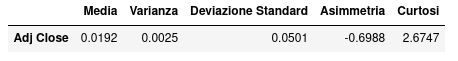
\includegraphics[width=1\linewidth]{goog_stats.png}
    \captionof{figure}{Statistiche univariate per Alphabet\\ (GOOG)}
    \label{fig:goog_stats}
  \end{minipage}%
  \begin{minipage}{.5\textwidth}
    \centering
    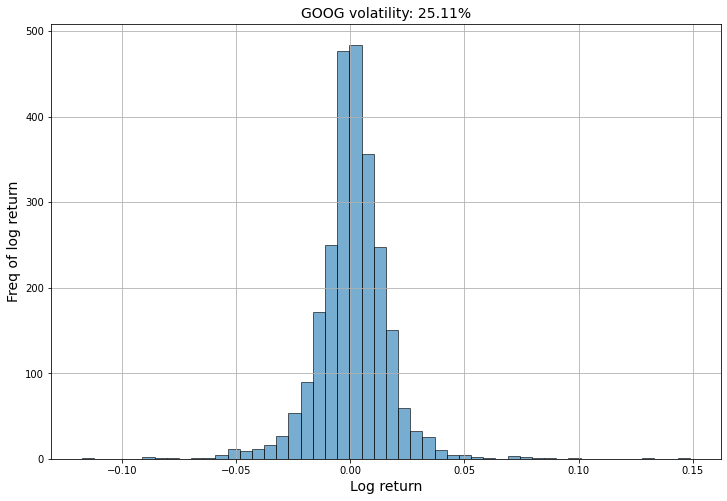
\includegraphics[width=1\linewidth]{goog_volatility.png}
    \captionof{figure}{Grafico volatilità di Alphabet (GOOG)}
    \label{fig:goog_vol}
  \end{minipage}
\end{figure}

\pagebreak

\textbf{Statistiche per Raytheon (RTX)}

Per Raytheon identifichiamo una volatilità del \verb|25.49|\%, i grafici e la tabella sono a figura \ref{fig:rtx_stats} e \ref{fig:rtx_vol}.

\begin{figure}[h]
  \centering
  \begin{minipage}{.5\textwidth}
    \centering
    \vspace{4.85cm}
    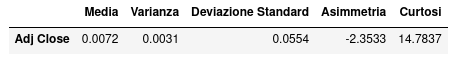
\includegraphics[width=1\linewidth]{rtx_stats.png}
    \captionof{figure}{Statistiche univariate per Raytheon\\ (RTX)}
    \label{fig:rtx_stats}
  \end{minipage}%
  \begin{minipage}{.5\textwidth}
    \centering
    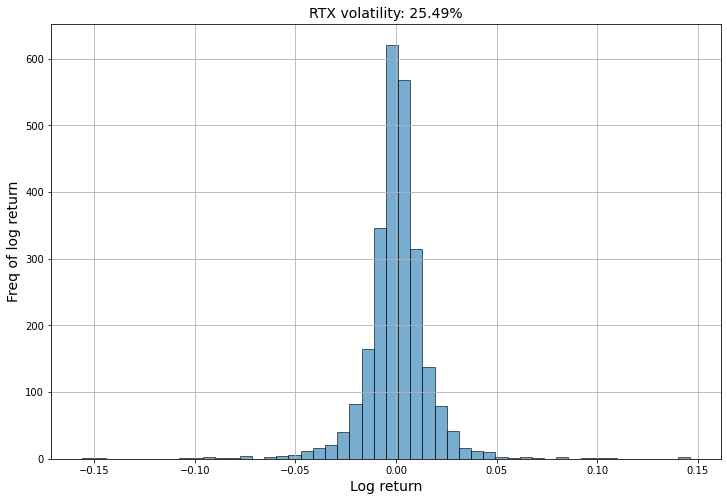
\includegraphics[width=1\linewidth]{rtx_volatility.png}
    \captionof{figure}{Grafico volatilità di Raytheon (RTX)}
    \label{fig:rtx_vol}
  \end{minipage}
\end{figure}

\textbf{Statistiche per Lockheed Martin (LMT)}

Per Lockheed Martin identifichiamo una volatilità del \verb|21.1|\%, i grafici e la tabella sono a figura \ref{fig:lmt_stats} e \ref{fig:lmt_vol}.

\begin{figure}[h]
  \centering
  \begin{minipage}{.5\textwidth}
    \centering
    \vspace{4.35cm}
    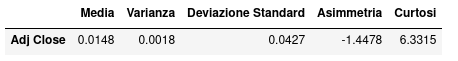
\includegraphics[width=1\linewidth]{lmt_stats.png}
    \captionof{figure}{Statistiche univariate per\\ Lockheed Martin (LMT)}
    \label{fig:lmt_stats}
  \end{minipage}%
  \begin{minipage}{.5\textwidth}
    \centering
    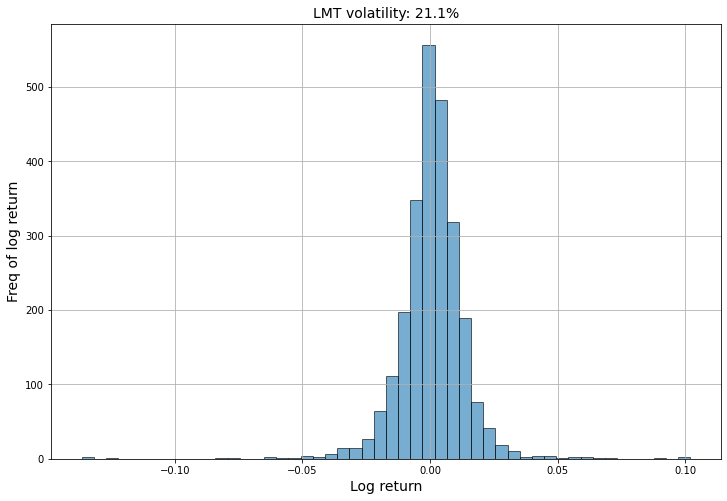
\includegraphics[width=1\linewidth]{lmt_volatility.png}
    \captionof{figure}{Grafico volatilità di Lockheed Martin (LMT)}
    \label{fig:lmt_vol}
  \end{minipage}
\end{figure}

\pagebreak

\textbf{Statistiche per Bank of America (BAC)}

Per Bank of America identifichiamo una volatilità del \verb|31.74|\%, i grafici e la tabella sono a figura \ref{fig:bac_stats} e \ref{fig:bac_vol}.

\begin{figure}[h]
  \centering
  \begin{minipage}{.5\textwidth}
    \centering
    \vspace{4.35cm}
    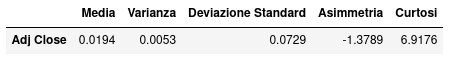
\includegraphics[width=1\linewidth]{bac_stats.png}
    \captionof{figure}{Statistiche univariate per\\ Bank of America (BAC)}
    \label{fig:bac_stats}
  \end{minipage}%
  \begin{minipage}{.5\textwidth}
    \centering
    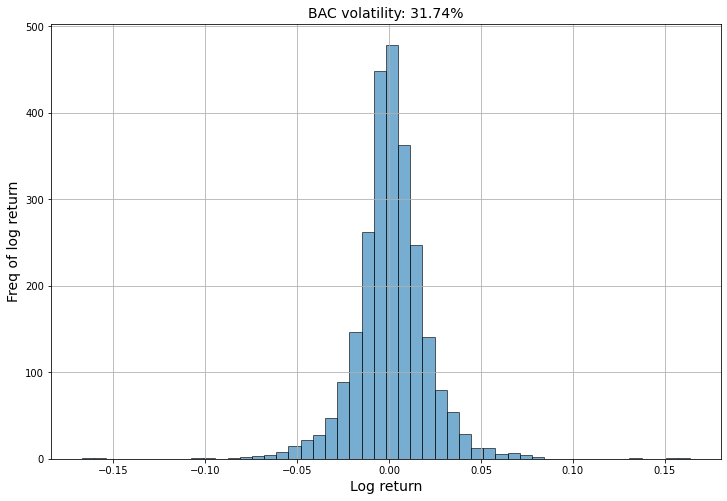
\includegraphics[width=1\linewidth]{bac_volatility.png}
    \captionof{figure}{Grafico volatilità di Bank of America (BAC)}
    \label{fig:bac_vol}
  \end{minipage}
\end{figure}

\textbf{Statistiche per JPMorgan Chase (JPM)}

Per JPMorgan  Chase identifichiamo una volatilità del \verb|27.04|\%, i grafici e la tabella sono a figura \ref{fig:jpm_stats} e \ref{fig:jpm_vol}.

\begin{figure}[h]
  \centering
  \begin{minipage}{.5\textwidth}
    \centering
    \vspace{4.35cm}
    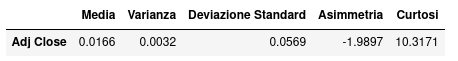
\includegraphics[width=1\linewidth]{jpm_stats.png}
    \captionof{figure}{Statistiche univariate per\\ JPMorgan Chase (JPM)}
    \label{fig:jpm_stats}
  \end{minipage}%
  \begin{minipage}{.5\textwidth}
    \centering
    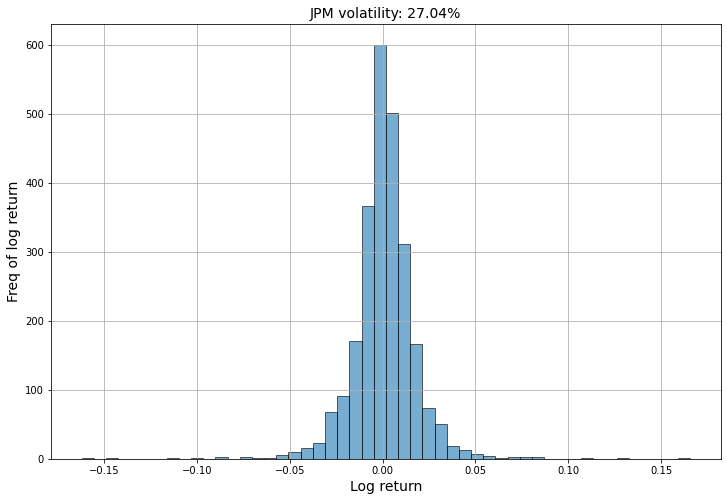
\includegraphics[width=1\linewidth]{jpm_volatility.png}
    \captionof{figure}{Grafico volatilità di JPMorgan Chase (JPM)}
    \label{fig:jpm_vol}
  \end{minipage}
\end{figure}

\bibliographystyle{alpha}
\bibliography{referenze}
\nocite{*}


\end{document}